%--------------------------------------------------------------------------------
\subsubsection{Synthetic CDO}
\label{ss:syntheticcdo} 

A synthetic CDS is priced in analogy to a CDS as the difference
between a premium leg value and a protection leg value. Key is 
the calculating of the {\em expected tranche loss} which affects both
the protection leg flow and valuation, and  remaining tranche notional 
that applies to the premium leg valuation.

\medskip
The total loss given default of the basket up to time $t$ is given by
$$
L(t) = \sum_{i=1}^N L^i(t),\qquad 
	L^i(t) = (1-R_i)\,N_i\,1_{\tau_i < t} 
$$ 
Where $N$ is the number of assets, and $1_{\tau_i < t}$ is the
indicator function that is equal to one if the time to default
$\tau_i$ for asset number $i$ is less than $t$. 
$L(t)$ is a random variable as the default times $\tau_i$.
 The tranche loss is then given by
$$ L_T(t) = \min(L(t),D) - \min(L(t),A) =  \left\{
  \begin{array}{ll}
  \displaystyle 0, & L(t) \leq A \\
  \displaystyle L(t) - A, & A < L(t) < D \\
  \displaystyle D - A, & L(t) \geq D
  \end{array}
  \right.
$$
 
The {\em expected tranche loss} is then calculated by integrating the 
tranche loss $L_T(t)$ over the probability density function $\rho(x)$
for loss $L(t)=x$
which can be shown to yield
\begin{align*} 
E[L_T(t)] &= \int_0^\infty dx \,(\min(x,D) - \min(x,A))\,\rho(x) \nonumber\\
 % &= \int_A^D dx \,(x-A)\,\rho(x) + (D-A)\int_D^\infty dx\, \rho(x) \nonumber\\
 % &= (D-A)\int_A^D dx \,\rho(x) - \int_A^D dx \int_A^x dx' \,\rho(x') + (D-A)\int_D^\infty dx\, \rho(x)  \nonumber\\
 % &= (D-A)\int_A^\infty \,dx\,\rho(x) - \int_A^D dx \int_A^x dx' \,\rho(x')  
 % 	\nonumber \\
 % &= (D-A) Pr\{L>A\} - \int_A^D dx \,Pr\{ A<L<x \} \nonumber \\
 % &= (D-A) Pr\{L>A\} - \int_A^D dx \,\left( 1 - Pr\{L<A\} - Pr\{L>x\} \right)
 % 	\nonumber \\
 &= \int_A^D\,dx \,Pr\{L(t)>x\} 
\end{align*}
and which shows that only {\em excess loss probability} $Pr\{L(t)>x\}$
is required to evaluate expected losses.
The present value of the expected payoff in time interval $[t_1, t_2]$
is then given by
$$
	\NPV_{t_1,t_2} = \left(E[L_T(t_2)] - E[L_T(t_1)]\right)\,P((t_1+t_2)/2), 
$$
and the present value of the entire protection leg by
$$ 
	\NPV_1 = \sum_{i=1}^N \left(E[L_T(t_i)] - E[L_T(t_{i-1})]\right)
		\,P((t_i+t_{i-1})/2) 
$$
where $P(t)$ is the discount factor for maturity $t$. 
Note that we assume that losses occur equally throughout the period 
so that discounting at the mid point is justified.  

The premium is paid on the protected notional amount, initially
$D-A$.  This notional is reduced by the expected protection payments 
$E_i$ at times $t_i$ so that the premium value is calculated as
$$ 
\NPV_2 = m \, \cdot \sum_{i=1}^N \,\left(D - A - E[L_T(t_i)]\right) 
	\cdot \delta_{i-1,i} \cdot P(t_i)
$$
where $m$ is the premium rate, $\delta_{i-1, i}$ is the day count
fraction between date/time $t_{i-1}$ and $t_i.$
The total CDO price for the protection seller is therefore
$\NPV=\NPV_2 - \NPV_1$. 

\bigskip
To compute the expected tranche loss for a basket that shows 
correlated defaults we use a single-factor Gaussian 
Copula model.

In the Copula approach, the individual assets' probability
distributions are glued together into a multivariate distribution that
introduces correlated default events. The Copula approach ensures by
construction that the marginal distributions recover each asset's
probability of default.

\medskip

Let $Q_i(t)$ be the cumulative probability that asset $i$ will default
before time $t$, i.e. the time of draw $t_i<t$. Evaluated at the
horizon $T$, $Q_i(T)=p_i$.

In a one-factor Copula model, consider random variables 
$$
 Y_i = a_i\,M+\sqrt{1-a_i^2}\:Z_i \label{y} 
$$
where $M$ and $Z_i$ have independent zero-mean unit-variance
distributions and $-1\leq a_i \leq 1$. The correlation between 
$Y_i$ and $Y_j$ is then $a_i a_j$.

Let $F_i(y)$ be the cumulative distribution function of $Y_i$. 
$y$ is mapped to $t$ such that percentiles match, i.e. 
$F_i(y)=Q_i(t)$ or $y=F_i^{-1}(Q_i(t))$.

Now let $H_i(z)$ be the cumulated distribution function of $Z_i$. 
For given realization of $M$, this determines the distribution of $y$:
$$ 
\P (y_i < y|M) = H \left( \frac{y-a_i\,M}{\sqrt{1-a_i^2}}\right) 
$$
or
$$
\P (t_i < t|M) = H \left( \frac{F_i^{-1}(Q_i(t))-a_i\,M}{\sqrt{1-a_i^2}}\right) 
$$

Let $G(m)$ be the cumulative distribution function of $M$, so that 
$g(m) = -\partial_m G(m)$ is its density: Integrating
over the density $g(m)$ yields the marginal probability of default for
 asset $i$
$$ 
Q_i(t) = \int_{-\infty}^\infty\, \P(t_i < t|M)\,g(m)\,dm 
= \int\, H \left( \frac{F_i^{-1}(Q_i(t))-a_i\,m}{\sqrt{1-a_i^2}}\right) \,g(m)\,dm.
$$

The loss distribution is now evaluated as follows:
\begin{itemize}
\item For each realization $m$ of $M$: evaluate the probability
  $p_i=Q_i(T)$ of default for each contract and
  determine the distribution of independent losses (conditional on $M$;
  for this purpose we use in general the {\em Hull-White Bucketing Algorithm}
  \cite{HullWhiteBucketing} as e.g. implemented in \cite{QuantLib}
  which allows for different individual $p_i$'s and loss associated loss
  amounts;  this yields $P_k(m)$ for all buckets $k$
\item Average the outcomes $P_k(m)$ for each bucket $k$ over the
  distribution of $M$
$$
P_k = \int_{-\infty}^\infty\,P_k(m)\,g(m)\,dm. \label{copula_2}
$$   
\end{itemize}

In a Gaussian copula model, $G$ and $H$ are set to the cumulative 
standard normal distribution. The integral above is
evaluated numerically, realizations of $M$ need not be generated with
Monte Carlo simulation. Note that the Gaussian distribution is stable
under convolution, i.e. also the distribution $F$ of $Y$ is Gaussian. 

% \subsubsection*{Student t Copula}
% This copula is based on the Student t distribution,
% $$
% f(t) = \frac{\Gamma((n+1)/2)}{\sqrt{n}\,\pi\,\Gamma(n/2)}\left(1+\frac{t^2}{n}\right)^{-(n+1)/2}
% $$
%  that has heavier tails than the Gaussian (and converges to a Gaussion
%  in the limit of $n\rightarrow\infty$). Its disadvantage is that the
%  distribution of $Y$ does not have an analytical expression even if
%  the distributions of $M$ and $Z$ are Student t distributions with
%  identical degrees of freedom $n$ - unlike the Gaussian, the Student t
%  distribution is not stable under convolution. The distribution of $Y$
%  needs to be computed numerically for each choice of the correlation
%  parameter.

Apart from discount curve, survival/default probability curves and
LGDs for each name in the basket we need copula correlations to
price  CDOs. These are quoted for equity tranches (attachment point
$A=0$) on indices such as iTraxx or CDX in the market, so-called {\em
  base correlations}. Any tranche can be priced as the difference of
two equity tranches with different detachment points and respective
base correlations. 

\subsubsection*{One-Factor Gaussian Copula Model with Stochastic Recovery}

To match IHS Markit methodology and prices we use a stochastic recovery extension of the
single-factor Gaussian Copula model above. The model is described in detail in 
\cite{Krekel_2008}. Here we provide a brief summary, aligning with the notation above:

Choose a discrete (marginal) recovery distribution for each entity $i$
conditioned on default ($\tau_i < t$)
$$
\widetilde R_i(t) = \left\{
\begin{array}{ccc} 
  r_{i,1} & \mbox{with probability} & p_{i,1} \\
  r_{i,2} & \mbox{with probability} & p_{i,2} \\
  \vdots & \vdots & \vdots \\
  r_{i,J} & \mbox{with probability} & p_{i,J} \\
\end{array}
  \right.
$$
with $r_{i,1} > r_{i,2} > \dots > r_{i,J}$
such that average/expected recovery rates match the quoted recovery rates:
$$  
\sum_{j=1}^J p_{i,j}\,r_{i,j} = R_i(t)
\qquad \mbox{and} \qquad
\sum_{j=1}^J p_{i,j} = 1.
$$

Now let $Q_{i,j}(t)$ be the cumulative probability of default of entity $i$
until $t$ with recovery rate less than $r_{i,j}$:
$$
Q_{i,j}(t) = Q_i(t) \cdot \sum_{k=j+1}^J p_{i,k}= Q_i(t) \cdot \left(1 - \sum_{k=1}^j p_{i,k}\right)
$$
so that
$$
0 = Q_{i,J} < Q_{i,J-1} < Q_{i,J-2} < \dots < Q_{i,0} = Q_i.
$$
Generalized thresholds for the factor $Y_i$ driving entity $i$'s default and its
recovery rate are now defined as
$$
C_{i,j}(t) = N^{-1}(Q_{i,j}(t))
$$
with
$$
-\infty = C_{i,J} < C_{i,J-1} < C_{i,J-2} < \dots < C_{i,1} < C_{i,0}.
$$
Entity $i$ is considered defaulted if variable $Y_i$ is less than threshold $C_{i,0}$
and it moreover defaults with recovery rate $r_{i,j}$ if $C_{i,j} < Y_i \leq C_{i,j-1}$.
$$
\qquad\qquad r_{i,J} < r_{i,J-1} < r_{i,J-2} < \dots < r_{i,1} 
$$
so that the highest recovery rate $r_{i,1}$ (lowest LGD) is associated with the region close to the default threshold $C_{i,0}$, as shown in figure \ref{fig_copula}.
\begin{figure}[htb]
\begin{center}
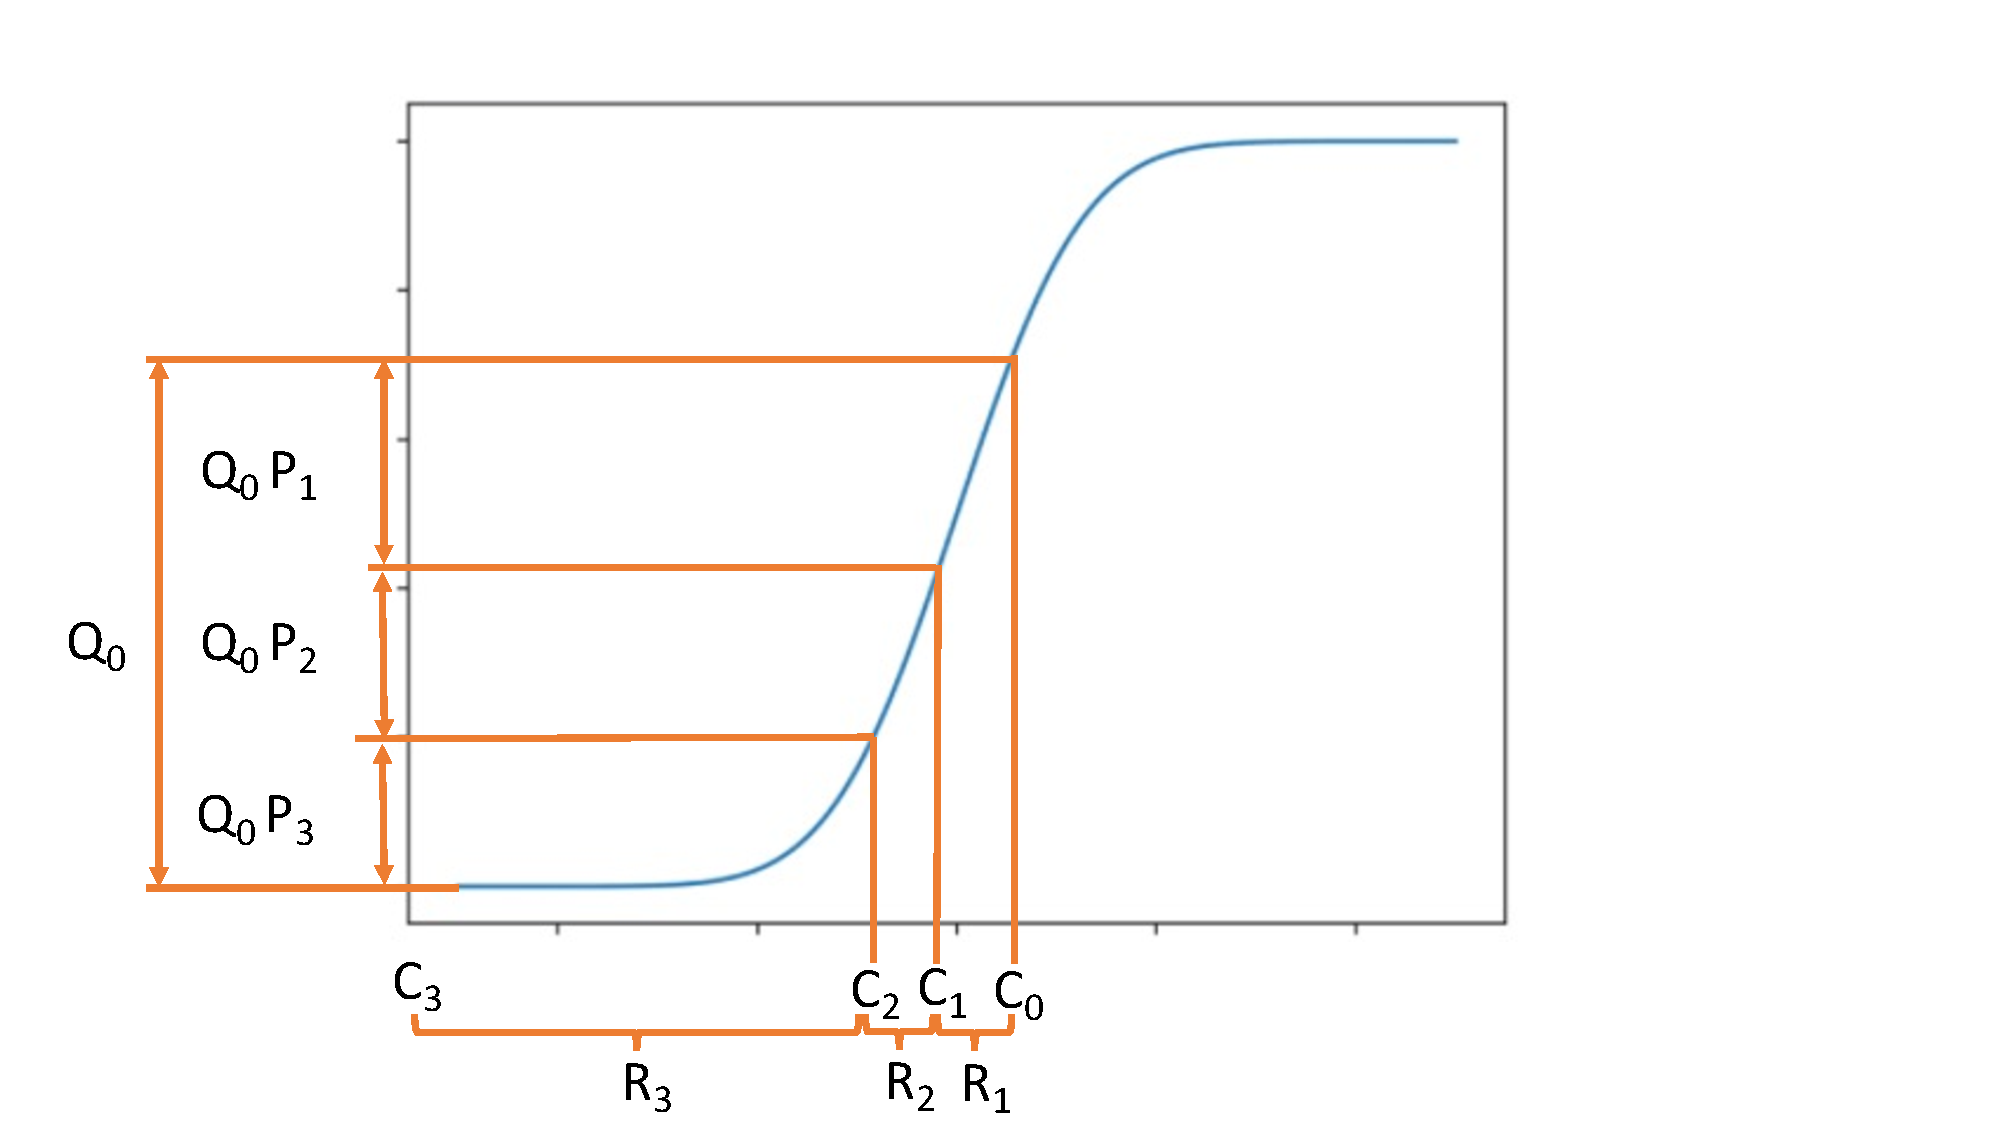
\includegraphics[scale=0.4]{pricing/cr_cdo_copula.pdf}
\end{center}
\caption{Probabilities, thresholds and recovery rates. }
\label{fig_copula}
\end{figure}

The Gaussian assumption for $Y_i$, $Z_i$ and $M$ then leads to the following probabilities
conditional on the common factor $M$:
\begin{itemize}
\item Probability of default
$$
P_i(M) := \P(t_i \leq t|M) = \P(Y_i \leq C_{i,0}(t)|M) = N \left( \frac{C_{i,0}(t) - a_i\,M}{\sqrt{1-a_i^2}}\right) 
$$
as in the standard Gaussian Copula case
\item Probability of recovery rate $r_{ij}$ given default of entity $i$
$$
  P_{i,j}(M) := \frac{\P(C_{i,j}(t) < Y_i \leq C_{i, j-1}(t) | M)}{\P(Y_i \leq C_{i,0}(t)|M)} 
  = \frac{ N \left( \frac{C_{i,j-1}(t) - a_i\,M}{\sqrt{1-a_i^2}}\right) - N \left( \frac{C_{i,j}(t) - a_i\,M}{\sqrt{1-a_i^2}}\right) }{ N \left( \frac{C_{i,0}(t) - a_i\,M}{\sqrt{1-a_i^2}}\right) }
  $$
\item Probability of default with recovery rate $r_{ij}$ 
  $$
  P_{i,j}(M)\times P_i(M) =  N \left( \frac{C_{i,j-1}(t) - a_i\,M}{\sqrt{1-a_i^2}}\right) - N \left( \frac{C_{i,j}(t) - a_i\,M}{\sqrt{1-a_i^2}}\right)
$$
\end{itemize}

The distribution of portfolio losses, conditional on $M$
$$
L(M) = \sum_{i=1}^N N_i\,(1-R_i(M))\,P_i(M) 
$$
is then computed by convolution. As in the single-recovery case we want to use a bucketing algorithm when loss amounts and default probabilities are allowed to differ across entities.
The {\em Hull-White Bucketing Algorithm} in \cite{HullWhiteBucketing} was extended slightly to handle the multi-recovery case.

\subsubsection{Calibration of default curves for index tranches}

If we calculate the npv of an Index CDS based on the underlying constituent CDS spread curves we notice a basis between the intrisinc value and the quoted index spread.
The basis and two methods to adjust the underlying curves to close the basis are described in detail in \cite{okane2008}.
Our calibration method is based on the idea of the Forward Default Probability Multiplier.

Instead of a calibration of the underlying curves to all quoted index terms in a iterative method and using a termstructure of adjustment factors, we are using a simpler method with a flat adjustment factor $\lambda$.

Let $Q_i(t)$ the survival probability of the i-th constituent at time t. Their adjusted survival probability is given by $\tilde{Q_i(t)}=Q_i(t)^\lambda$.

When we are pricing a index CDS tranche, we set the factor $\lambda$ so that the intrinsic valuation of the underlying index CDS with the adjusted curves matches the quoted price.




